\documentclass[12pt]{article}
\usepackage{titlesec}
\usepackage{subcaption}
\usepackage[scaled]{helvet}  \renewcommand\familydefault{\sfdefault} % Font
\usepackage{graphicx} % Required for inserting images
\usepackage{geometry}
\usepackage[colorlinks=true, urlcolor=blue, linkcolor=red]{hyperref}
\usepackage{pgfplotstable}
\usepackage{amsmath}
\usepackage{enumitem}
\usepackage{tikz} 
\usetikzlibrary{petri,arrows.meta}
\geometry{a4paper, total={170mm,257mm},left=20mm, top=20mm,}
\usepackage[listings,breakable,skins]{tcolorbox}
% declare our code block environment
  \newtcblisting{tcbcodeblock}[1]{%
    enhanced,
    sharp corners,
    colframe=black,
    coltext=codefg,
    colback=codebg,
    breakable,
    size=fbox,
    listing only,
    listing options={%
      style=tcblatex,
      language={#1},
      showspaces=false,
      showstringspaces=false,
      commentstyle=\color{codegray},
      keywordstyle=\color{codegreen},
      stringstyle=\color{codecyan},
      basicstyle=\ttfamily\footnotesize
    }
  }
\renewcommand{\thesection}{\Roman{section}}
\renewcommand{\thesubsection}{\arabic{subsection}}
\renewcommand{\thesubsubsection}{\alph{subsubsection}.}

\titleformat{\section}{\normalfont\LARGE\bfseries}{\thesection.}{10pt}{}
\titleformat{\subsection}{\normalfont\Large}{\thesubsection.}{10pt}{}
\titleformat{\subsubsection}{\normalfont\large}{\thesubsubsection}{10pt}{}

\begin{document}
\thispagestyle{empty} %Suppress number of this page
\begin{center}
    \vspace{7pt}
    \fontsize{18pt}{17pt}\selectfont 
    \textbf{University of Science and Technology of Hanoi}
    \vspace{7pt}
\end{center}
\vspace{10pt}
\begin{center}
    
\includegraphics[scale=0.4]{USTH.png}
\end{center}

\vspace{90pt}

\begin{center}
    \fontsize{30pt}{17pt}\selectfont 
    \textbf{Subject} 
    \vspace{50pt}

    \fontsize{20pt}{17pt}\selectfont 
    \textbf{Advanced programming HPC Labwork 3}
    \vspace{50pt}


    \fontsize{17pt}{17pt}\selectfont
    \textbf{{Student id: }{ict2440050}}
    \vspace{15pt}

    \fontsize{17pt}{17pt}\selectfont
    \textbf{{Student name: }{Nguyen Vu Bach}}
    \vspace{15pt}
    
\end{center}

\newpage
\setcounter{page}{1} % Start number from this page
\section{Load image}
\begin{figure}[h!]
    \centering
    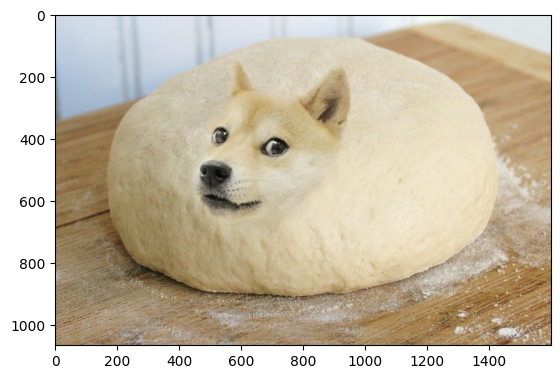
\includegraphics[width=0.75\linewidth]{Original.png}
    \caption{Original image}
    \label{fig:placeholder}
\end{figure}

The image shape \((1065, 1600, 3)\) is downloaded from a random place on the internet as JPG and loaded using \(matplotlib.pyplot.imread\). 

\section{Flatten image}
Image is flatten into 1D by reshape with pixel count where pixel count is calculated by:
\begin{equation}
    pixel\_count = height * width
\end{equation}
The image after reshape has a shape of \((1704000, 3)\)


\newpage
\section{Grayscale}
There was an attempt to do grayscale on local laptop but I can not fix the "[1] 21385 segmentation fault (core dumped)" problem. It could either be cudatoolkit version incompatible or GPU lack of VRAM.

\subsection{With CPU}
\begin{figure}[h!]
    \centering
    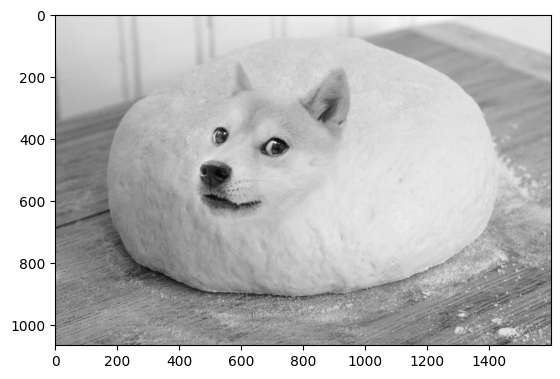
\includegraphics[width=0.75\linewidth]{CPU.png}
    \caption{CPU grayscale image}
    \label{fig:placeholder}
\end{figure}
Grayscale using equation from \href{https://stackoverflow.com/questions/69424054/converting-bgr-image-to-grayscale-using-numpy}{stackoverflow}, the equation state as follow:
\begin{equation}
    img\_gray = (0.2989 * r + 0.5870 * g + 0.1140 * b)
\end{equation}

The process took 12.7815 seconds to finish.

\subsection{With GPU}
\begin{figure}[h!]
    \centering
    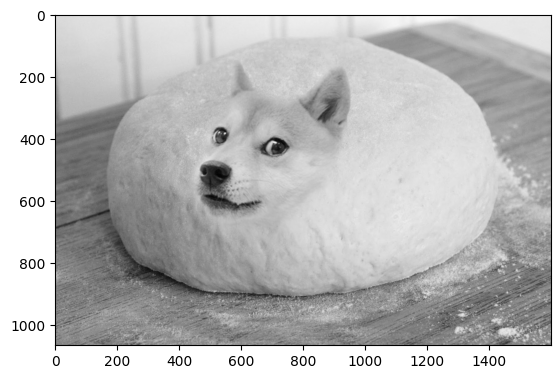
\includegraphics[width=0.75\linewidth]{GPU.png}
    \caption{GPU grayscale image}
    \label{fig:placeholder}
\end{figure}

The grid size equation is taken from \href{https://github.com/dinonomous/GPU-Accelerated-Image-Grayscale/blob/main/cuda_grayscale_colab.py}{this github}
\begin{equation}
    grid\_size = \frac{(pixel\_count + (block\_size - 1))}{block\_size}
\end{equation}

\newpage



\begin{figure}[h!]
    \centering
    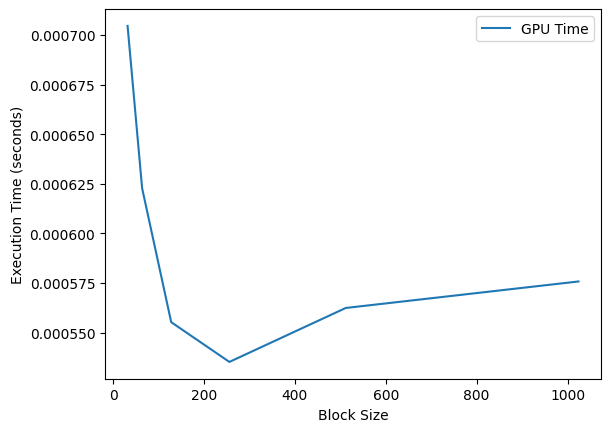
\includegraphics[width=0.75\linewidth]{Plot.png}
    \caption{Block Size vs Execution Time}
    \label{fig:placeholder}
\end{figure}

I experiment with different block sizes [32, 64, 128, 256, 512, 1024]. Although, I think that the experiment is actually not accurate since cuda cache should be reset after each run.

\end{document}







